\section{Resultados}

Este tópico é dedicado a apresentar os resultados, adversidades e contribuições 
alcançadas durante o desenvolvimento do estudo referente ao problema proposto. 
Por fim, são apresentadas considerações sobre as limitações ocorridas no 
desenvolvimento deste trabalho. Nos resultados do problema proposto, este 
estudo utilizou as principais métricas da literatura para análise de desempenho 
dos classificadores.

\subsection{Configuração do experimento}

Dada a matriz de referência do \citeauthor{edital_enem:2016} 
(\citeyear{edital_enem:2016}), a competência III foi selecionada 
aleatóriamente como o alvo da inferência indutiva dos classificadores.

\subsection{Disposição das classes no \textit{dataset}}

Dada as 6.663 redações coletadas originalmente, com temas diversificados que 
passaram em um processo de avaliação manual com diferentes avaliadores, a 
aplicação dos métodos de balanceamento e limpeza de dados, filtrou um segundo 
\textit{dataset}, dispondo de 690 redações. O Gráfico 
\ref{graphic:dataset_balanced} demonstra a disposição das classes distintas 
(0.00, 0.50, 1.00, 1.50, 2.00) sobre as cinco competências exigidas.

\begin{figure}[H]
    \begin{center}
    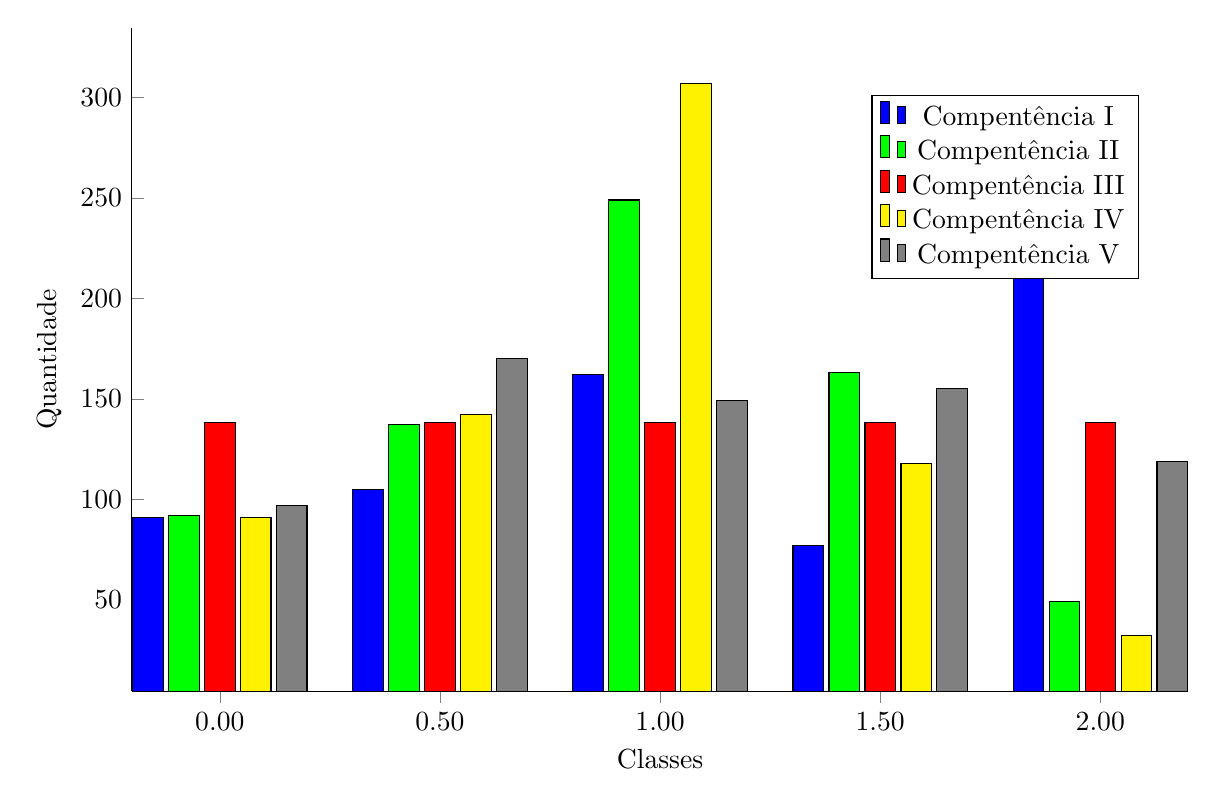
\begin{tikzpicture}
        \begin{axis}[
                ybar,
                width=15cm,
                height=10cm,
                symbolic x coords={0.00,0.50,1.00,1.50,2.00},
                legend style={at={(0.7,0.9)},anchor=north west},
                bar width=11pt,
                ylabel=Quantidade,
                xlabel=Classes,
                xtick=data,
                axis lines*=left,
            ]
            \addlegendentry{Compentência I}
            \addplot[draw=black, fill=blue] coordinates{
                (0.00,91)
                (0.50,105)
                (1.00,162)
                (1.50,77)
                (2.00,255)
            };

            \addlegendentry{Compentência II}
            \addplot[draw=black, fill=green] coordinates{
                (0.00,92)
                (0.50,137)
                (1.00,249)
                (1.50,163)
                (2.00,49)
            };

            \addlegendentry{Compentência III}
            \addplot[draw=black, fill=red] coordinates{
                (0.00,138)
                (0.50,138)
                (1.00,138)
                (1.50,138)
                (2.00,138)
            };

            \addlegendentry{Compentência IV}
            \addplot[draw=black, fill=yellow] coordinates{
                (0.00,91)
                (0.50,142)
                (1.00,307)
                (1.50,118)
                (2.00,32)
            };

            \addlegendentry{Compentência V}
            \addplot[draw=black, fill=gray] coordinates{
                (0.00,97)
                (0.50,170)
                (1.00,149)
                (1.50,155)
                (2.00,119)
            };

            % \node [above] at (axis cs:  0.00,138) {138};
            % \node [above] at (axis cs:  0.50,138) {138};
            % \node [above] at (axis cs:  1.00,138) {138};
            % \node [above] at (axis cs:  1.50,138) {138};
            % \node [above] at (axis cs:  2.00,138) {138};
        \end{axis}
    \end{tikzpicture}
    \caption{Distribuição das classes sobre a competência III de 690 redações 
    no \textit{dataset} balanceado, cada classe da competência III possui uma 
    amostragem de 138 redações.}
    \label{graphic:dataset_balanced}
    \end{center}
\end{figure}

A quantidade de exemplos da competência III obtidos no \textit{dataset} pode 
apresentar-se de uma certa forma modesta, entretanto normalmente é 
suficientemente para produzir resultados relevantes na validação cruzada.

\subsection{Resultado da inferência indutiva}

A inferência indutiva dos classificadores \textit{Adabost} e 
\textit{Naive Bayes}, utilizando o \textit{dataset} originou o Gráfico 
\ref{graphic:acuracia}, onde está delineado os resultados da 
\textit{acurácia} de cada classe distinta sobre domínio do problema. Com isso, 
nota-se que em relação ao algoritmo \textit{Adaboost}, a indução do 
\textit{Naive Bayes} proveu uma melhor acurácia na maior parte das classes.

% Acurácia
\begin{figure}[H]
    \begin{center}
        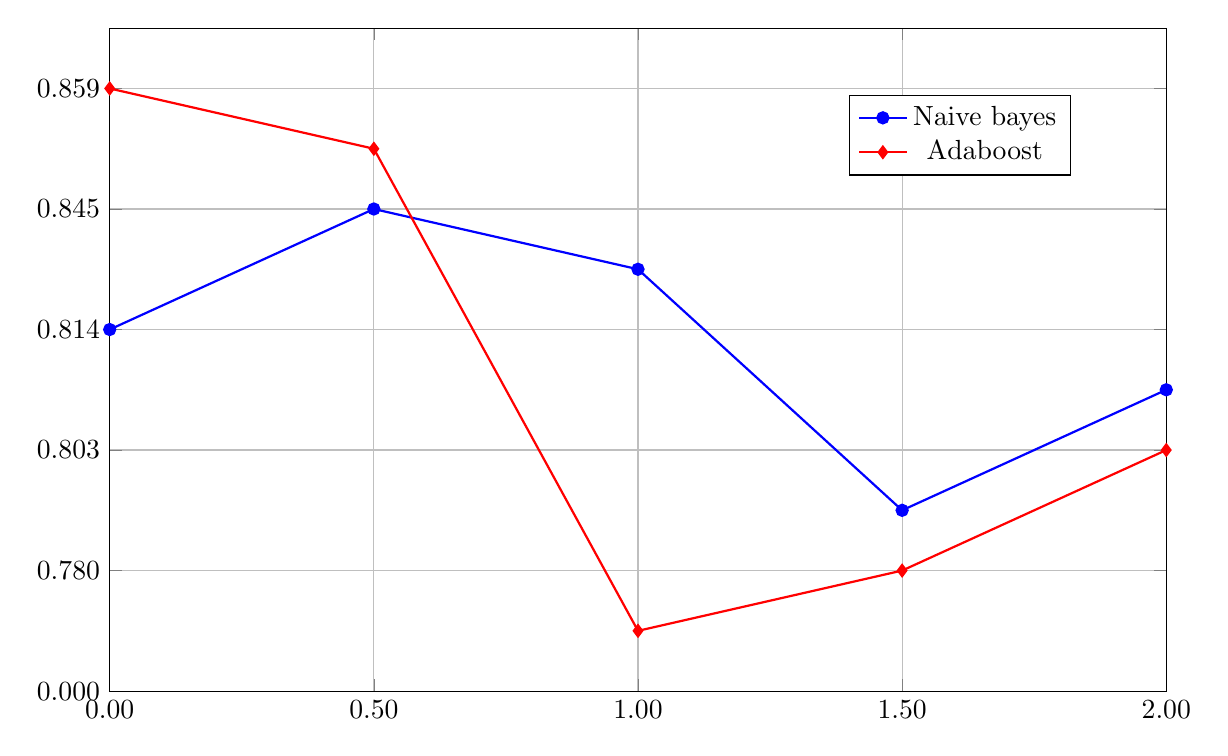
\begin{tikzpicture}
        \begin{axis}[width=15cm, 
            height=10cm, 
            grid=both, 
            ymin=0.000,
            ymax=0.900,
            xmax=2.00,
            xmin=0.00, 
            legend style={at={(0.7,0.9)},anchor=north west},
            symbolic x coords={0.00, 0.50, 1.00, 1.50, 2.00}, 
            symbolic y coords={0.000, 0.770,0.780,0.791,0.803,0.810,0.814,0.817,0.845,0.858,0.859, 0.900},
            xtick=data]

        \addlegendentry{Naive bayes}
        \addplot[mark=*,thick,blue] coordinates {
        (0.00,0.814) 
        (0.50,0.845) 
        (1.00,0.817) 
        (1.50,0.791) 
        (2.00,0.810) 
        };

        \addlegendentry{Adaboost}
        \addplot[mark=diamond*,thick,red] coordinates {
        (0.00,0.859) 
        (0.50,0.858) 
        (1.00,0.770) 
        (1.50,0.780) 
        (2.00,0.803) 
        };

        \end{axis}
        \end{tikzpicture}
    \end{center}
    \caption{Sobreposição dos resultados de \textit{acurácia} na inferência  
    indutiva dos algoritmos \textit{Adaboost} e \textit{Naive Bayes}.}
    \label{graphic:acuracia}
\end{figure}

No Gráfico \ref{graphic:roc} é apresentado os resultados referentes 
ao ponto de corte da curva ROC correspondente a cada classe distinta. Através 
deste ponto avalia-se que o poder de discriminação das classes do algoritmo 
\textit{Naive Bayes} foi superior em relação ao \textit{Adaboost}. 

% Curva ROC
\begin{figure}[H]
    \begin{center}
        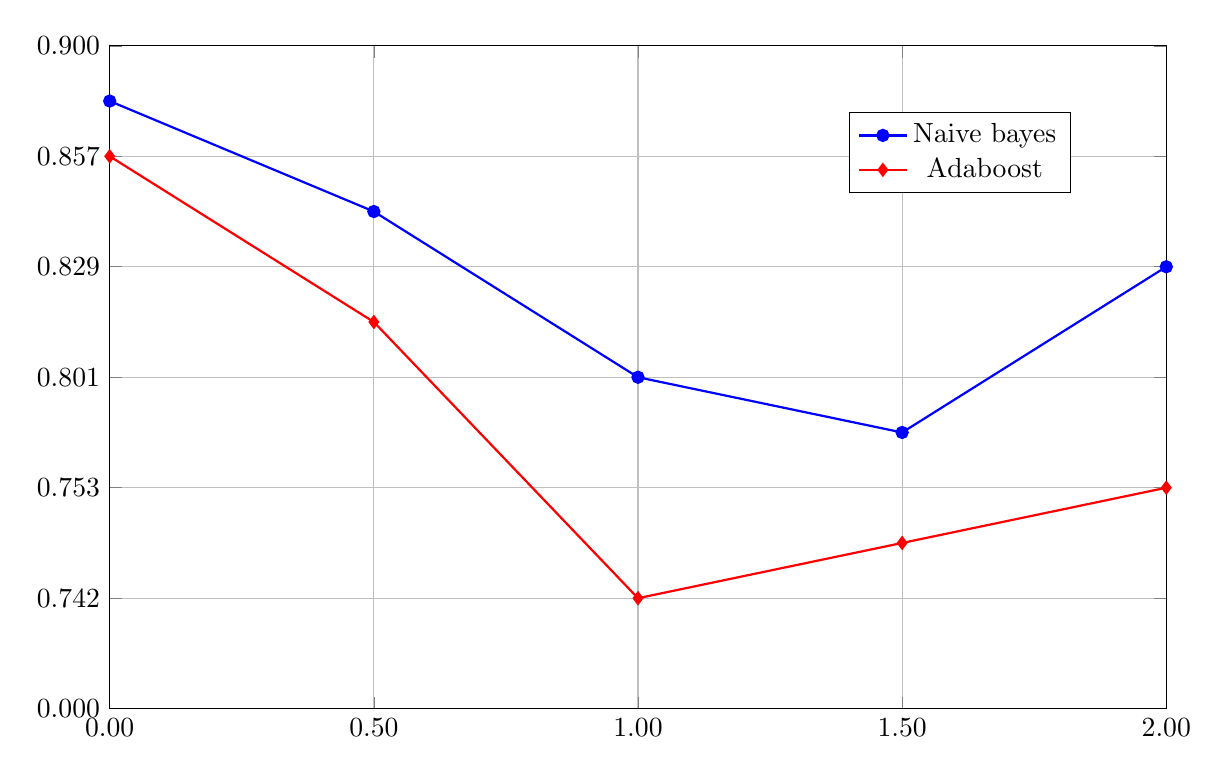
\begin{tikzpicture}
        \begin{axis}[width=15cm, 
            height=10cm, 
            grid=both, 
            ymin=0.000,
            ymax=0.900,
            xmax=2.00,
            xmin=0.00, 
            legend style={at={(0.7,0.9)},anchor=north west},
            symbolic x coords={0.00, 0.50, 1.00, 1.50, 2.00}, 
            symbolic y coords={0.000, 0.500, 0.742,0.752,0.753,0.795,0.801,0.810,0.829,0.851,0.857,0.868, 0.900},
            xtick=data]

        \addlegendentry{Naive bayes}
        \addplot[mark=*,thick,blue] coordinates {
        (0.00,0.868) 
        (0.50,0.851) 
        (1.00,0.801) 
        (1.50,0.795) 
        (2.00,0.829) 
        };

        \addlegendentry{Adaboost}
        \addplot[mark=diamond*,thick,red] coordinates {
        (0.00,0.857) 
        (0.50,0.810) 
        (1.00,0.742) 
        (1.50,0.752) 
        (2.00,0.753) 
        };

        \end{axis}
        \end{tikzpicture}
    \end{center}
    \caption{Sobreposição dos resultados da curva ROC na inferência 
    indutiva dos algoritmos \textit{Adaboost} e \textit{Naive Bayes}.}
    \label{graphic:roc}
\end{figure}

A matriz de confusão ou tabela de contingência é uma ferramenta importante para 
avaliar os resultados da predição, facilita visualmente o entendimento e reage 
aos efeitos de predições falsas.

% Matriz de confusão Naive Bayes
\begin{table}[H]
    \centering
    \begin{tabular}{cc|c|c|c|c|c|c|}
    \cline{3-8}
     &  & \multicolumn{6}{c|}{\textbf{Naive Bayes}} \\ \cline{3-8} 
     &  & \textbf{0.00} & \textbf{0.50} & \textbf{1.00} & \textbf{1.50} & \textbf{2.00} & $\sum_{}$  \\ \hline
    \multicolumn{1}{|c|}{} & \textbf{0.00} & \textbf{92} & 23 & 9  & 6  & 8  & \textit{138} \\ \cline{2-8} 
    \multicolumn{1}{|c|}{} & \textbf{0.50} & 20 & \textbf{83} & 28 & 4  & 3  & \textit{138} \\ \cline{2-8} 
    \multicolumn{1}{|c|}{} & \textbf{1.00} & 24 & 18 & \textbf{68} & 19 & 9  & \textit{138} \\ \cline{2-8} 
    \multicolumn{1}{|c|}{} & \textbf{1.50} & 19 & 5  & 12 & \textbf{75} & 27 & \textit{138} \\ \cline{2-8} 
    \multicolumn{1}{|c|}{} & \textbf{2.00} & 19 & 6  & 7  & 52 & \textbf{54} & \textit{138} \\ \cline{2-8} 
    \multicolumn{1}{|c|}{\multirow{-6}{*}{\rot{Atual}}} & $\sum_{}$ & \textit{172} & \textit{135} & \textit{124} & \textit{156} & \textit{101} & \textit{690} \\ \hline
    \end{tabular}
    \caption{Matriz de confusão resultante da indução do classificador Naive Bayes.}
    \label{tab:matrix_naive_bayes}
\end{table}

% Matriz de confusão Adaboost
\begin{table}[H]
    \centering
    \begin{tabular}{cc|c|c|c|c|c|c|}
    \cline{3-8}
     &  & \multicolumn{6}{c|}{\textbf{Adaboost}} \\ \cline{3-8} 
     &  & \textbf{0.00} & \textbf{0.50} & \textbf{1.00} & \textbf{1.50} & \textbf{2.00} & $\sum_{}$  \\ \hline
    \multicolumn{1}{|c|}{} & \textbf{0.00} & \textbf{83} & 10 & 27 & 11 & 7  & \textit{138} \\ \cline{2-8} 
    \multicolumn{1}{|c|}{} & \textbf{0.50} & 17 & \textbf{74} & 38 & 8  & 1  & \textit{138} \\ \cline{2-8} 
    \multicolumn{1}{|c|}{} & \textbf{1.00} & 10 & 19 & \textbf{77} & 19 & 13 & \textit{138} \\ \cline{2-8} 
    \multicolumn{1}{|c|}{} & \textbf{1.50} & 3  & 2  & 21 & \textbf{74} & 38 & \textit{138} \\ \cline{2-8} 
    \multicolumn{1}{|c|}{} & \textbf{2.00} & 12 & 3  & 12 & 50 & \textbf{61} & \textit{138} \\ \cline{2-8} 
    \multicolumn{1}{|c|}{\multirow{-6}{*}{\rot{Atual}}} & $\sum_{}$ & \textit{125} & \textit{108} & \textit{175} & \textit{162} & \textit{120} & \textit{690} \\ \hline
    \end{tabular}
    \caption{Matriz de confusão resultante da indução do classificador Adaboost.}
    \label{tab:matrix_adaboost}
\end{table}

A análise da matriz na Tabela 
\ref{tab:matrix_naive_bayes} e \ref{tab:matrix_adaboost} respectivamente dos 
algoritmos \textit{Naive Bayes} e \textit{Adaboost} foi fundamental para a
avaliação dos classificadores. Em ambos classificadores o resultado poderia ser 
melhor, se caso o padrão encontrado dentro do texto pudessem ser mensurado com 
maior representatividade obtendo uma melhor separação entre as valorações de 
cada competência, entretanto este resultado corrobora com a hipótese proposta 
para este estudo. De acordo ainda com a análise da matriz de confusão 
apresentada nas Tabelas \ref{tab:matrix_naive_bayes} e 
\ref{tab:matrix_adaboost}, o número de predições corretas do classificador 
\textit{Naive Bayes} apresentou um resultado melhor em relação 
ao algoritmo \textit{Adaboost}. 
